\chapter{Methodology}
\label{chap:methodology}

\lettrine[lines=3, findent=3pt, nindent=0pt]{C}{hapter} 3 deals with software and methodologies used for building the \gls{ids}. Starting with the concept behind the code, will then be discussed the scripts used, the pre-processing done to the chosen dataset, along with some statistics about the latter and the algorithms adopted in the \gls{ml} model training. In the final section will also be provided a \gls{poc} to demonstrate the functioning of the final product. The workflow has revolved around Git as \gls{vcs}\footnote{See appendix \ref{app:repository}}.

%----------------------------------------------------
% CONCEPT
%----------------------------------------------------

\section{Concept}
\label{sec:concept}

In this section will be explained the more abstract and high-level idea, on which the \gls{ids} was built. The concept is summarized by the following figure:

\begin{figure}[h!]
    \centering
    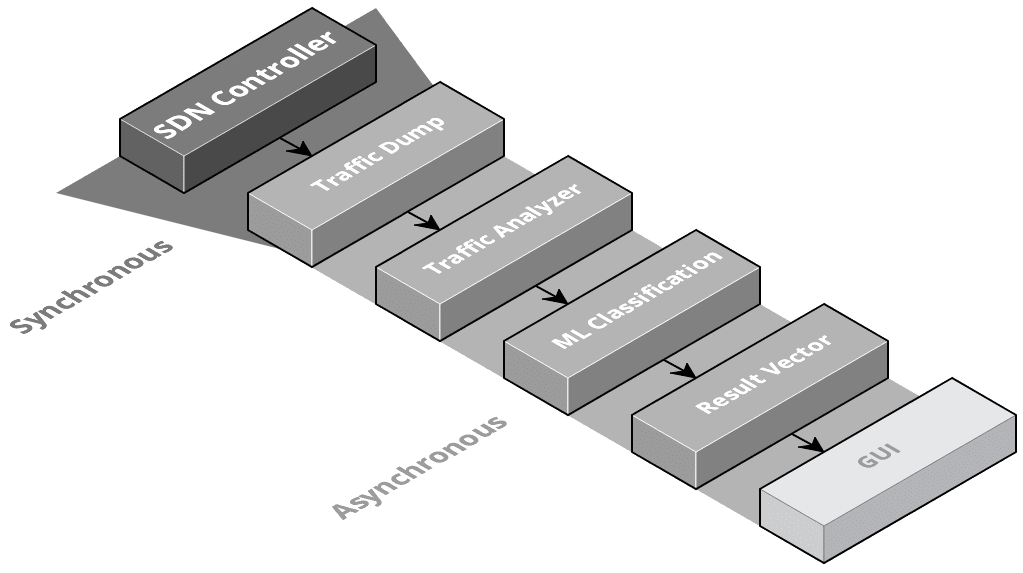
\includegraphics[scale=0.32]{assets/figures/chapter3/concept-components.png}
    \caption{Project's flowchart: from raw traffic to classified vector}
    \label{fig:concept-components}
\end{figure}

\noindent The system can be used in both, \textit{synchronous} or \textit{asynchronous} mode. Proceeding top-down, the \textit{SDN Controller} serves the purpose of orchestrating the duplication of network traffic\footnote{See section \ref{subsubsec:traffic-duplication}} in order to create a \gls{pcap} file (so called \textit{traffic dump}) every some amount of seconds (chosen by the user). The latter will be than passed to the \textit{Analyzer}, which has the task of converting the traffic dump into a vector and pass it to the \gls{ml} model, in order to perform classification. The Analyzer can also get user uploaded files as input, and this allows the asynchronous operation. The \textit{\gls{ml} Classification} block consists of passing the previously mentioned vector to the trained \gls{rf} model and appending periodically the results to a \glsxtrshort{csv} file. In the final step, the \textit{Result Vector} can be visualized using the web \gls{gui}.

%----------------------------------------------------
% MODEL TRAINING
%----------------------------------------------------

\section{Machine Learning Model Training}
\label{sec:model-training}

This is the first stage of the implementation. For this purpose was used a \textit{Jupyter Notebook} to pre-process and visualize the raw data and then to train the \gls{ml} model. For reference, all the operations described were done using a MacBook Pro with 8 GB of RAM and an iMac with 16 GB of RAM, both running macOS 11.4 (Big Sur). The datasets used, as discussed in \ref{subsec:datasets-for-evaluation}, are NSL-KDD and CICIDS2017. The former was only used to become familiar with \gls{ml} and Jupyter Notebooks in general, the latter was the one strictly useful to the project.

%----------------------------------------------------
% PRE-PROCESSING
%----------------------------------------------------

\subsection{Pre-Processing}
\label{subsec:pre-processing}

After the dataset choice, \textit{pre-processing} is very important in order to get consistent results regarding the training of the \gls{ml} model, and so the accuracy of the \gls{ids}. It is important to remove redundant or null records and unimportant features. The dataset used contains plenty records so \texttt{NaN}, \texttt{Null} and \texttt{Inf} values were dropped to clean the data the model will work with. Also columns containing non numerical values were dropped (\texttt{Flow\_ID}, \texttt{Source\_IP}, \texttt{Destination\_IP}, \texttt{Timestamp}), except the one containing the traffic category (\texttt{Label}). \\ In order to visualize and comprehend what is going on, Python's \textit{Pandas Library} \cite{PandasLibrary} was the choice. Printing the dataset's value counts helps to understand the ratio between normal traffic and malicious one. 

\begin{table}[h!]
    \centering
    \begin{tabular}{l|l}
        \toprule 
        Traffic Label & Entries \\
        \midrule
        \rowcolor{black!10} Benign & 2,271,320 \\
        DoS Hulk & 230,124 \\
        \rowcolor{black!10} Port Scan & 158,804 \\
        DDoS & 128,025 \\
        \rowcolor{black!10} DoS GoldenEye & 10,293 \\
        FTP-Patator & 7,935 \\
        \rowcolor{black!10} SSH-Patator & 5,897 \\
        DoS Slowloris & 5,796 \\
        \rowcolor{black!10} DoS Slowhttptest & 5,499 \\
        Bot & 1,956 \\
        \rowcolor{black!10} Web Attack: Brute Force & 1,507 \\
        Web Attack: XSS & 652 \\
        \rowcolor{black!10} Infiltration & 36 \\
        Web Attack: SQL Injection & 21 \\
        \rowcolor{black!10} Heartbleed & 11 \\
        \bottomrule
    \end{tabular}
    \caption{CICIDS2017 (ungrouped) Value Counts}
    \label{tab:dataset-distribution}
\end{table}

\noindent From the above table comes clear that there are traffic categories with insufficient data to train the model, and have to be dropped (Infiltration, SQL Injection and Heartbleed). The remaining 12 labels were than grouped by relevance according to the table below, in order to generalize the categorization.

\begin{table}[h!]
    \centering
    \begin{tabular}{l|l|l}
        \toprule 
        Group Name & Labels & Entries \\
        \midrule
        \rowcolor{black!10} Benign & Benign & 2,271,320 \\
        Dos & DoS Hulk, DoS GoldenEye, DoS Slowloris, DoS Slowhttptest &  251,712 \\
        \rowcolor{black!10}Probe & Port Scan & 158,804 \\
        DDoS & DDoS & 128,025 \\
        \rowcolor{black!10}Brute Force & FTP-Patator, SSH-Patator  & 13,832 \\
        Web Attack & Web Attack: Brute Force, Web Attack: XSS & 2,159 \\
        \rowcolor{black!10}Botnet & Bot & 1,956 \\
        \bottomrule
    \end{tabular}
    \caption{CICIDS2017 (grouped) Value Counts}
    \label{tab:grouped-dataset-distribution}
\end{table}

\noindent Another step of the pre-processing stage consisted in splitting the dataset. Being the latter explicitly unbalanced, since it consists in 5 days of traffic acquisition, each one dedicated to a specific attack type, it was performed a \textit{stratified split}, using Pandas' \texttt{train\_test\_split()}, which splits arrays or matrices into train and test subsets, maintaining the same ratio of classes across the subsets. As pointed out in \cite{Mozley2020}, a fundamental step in pre-processing is \textit{normalization}: since the scale of the feature value differs, to ensure that each one of them contribute the same amount to the classification, it is mandatory to bring them to the same range. In Python it is possible to do a \textit{min-max normalization} using \texttt{scikit-learn} library \cite{ScikitWebsite}. This kind of operation re-scales the dataset's features using the following equation:

\begin{equation}
    x\prime=\frac{x-\min\{x\}}{\max\{x\}-\min\{x\}}
\end{equation}
In which $x$ is the feature's original value.

%----------------------------------------------------
% FEATURES AND STATISTICS
%----------------------------------------------------

\subsection{Features and Statistics}
\label{subsec:features-statistics}

As pointed out in \ref{subsec:traffic-characterization}, given a dataset, some features are more relevant than others. In order to achieve an higher accuracy and generalization and saving time in the training stage, the right move was using only the most relevant features in such a fashion that if the feature value and the class label are independent, then the elder is not relevant in the classification process, therefore it has to be dropped. The library of choice was \texttt{scikit-learn} \cite{ScikitWebsite}, and in particular it's \texttt{SelectKBest} function: this was helpful for selecting the top 40 (in this particular case) most dependent features of the dataset, using the \textit{chi-squared} algorithm. The chart below represents a plot of the features score mentioned earlier: to be noticed is the dotted line, which represents the $99\%$ mark, meaning that all the features above are not so relevant for the purpose.

\begin{figure}[h!]
    \centering
    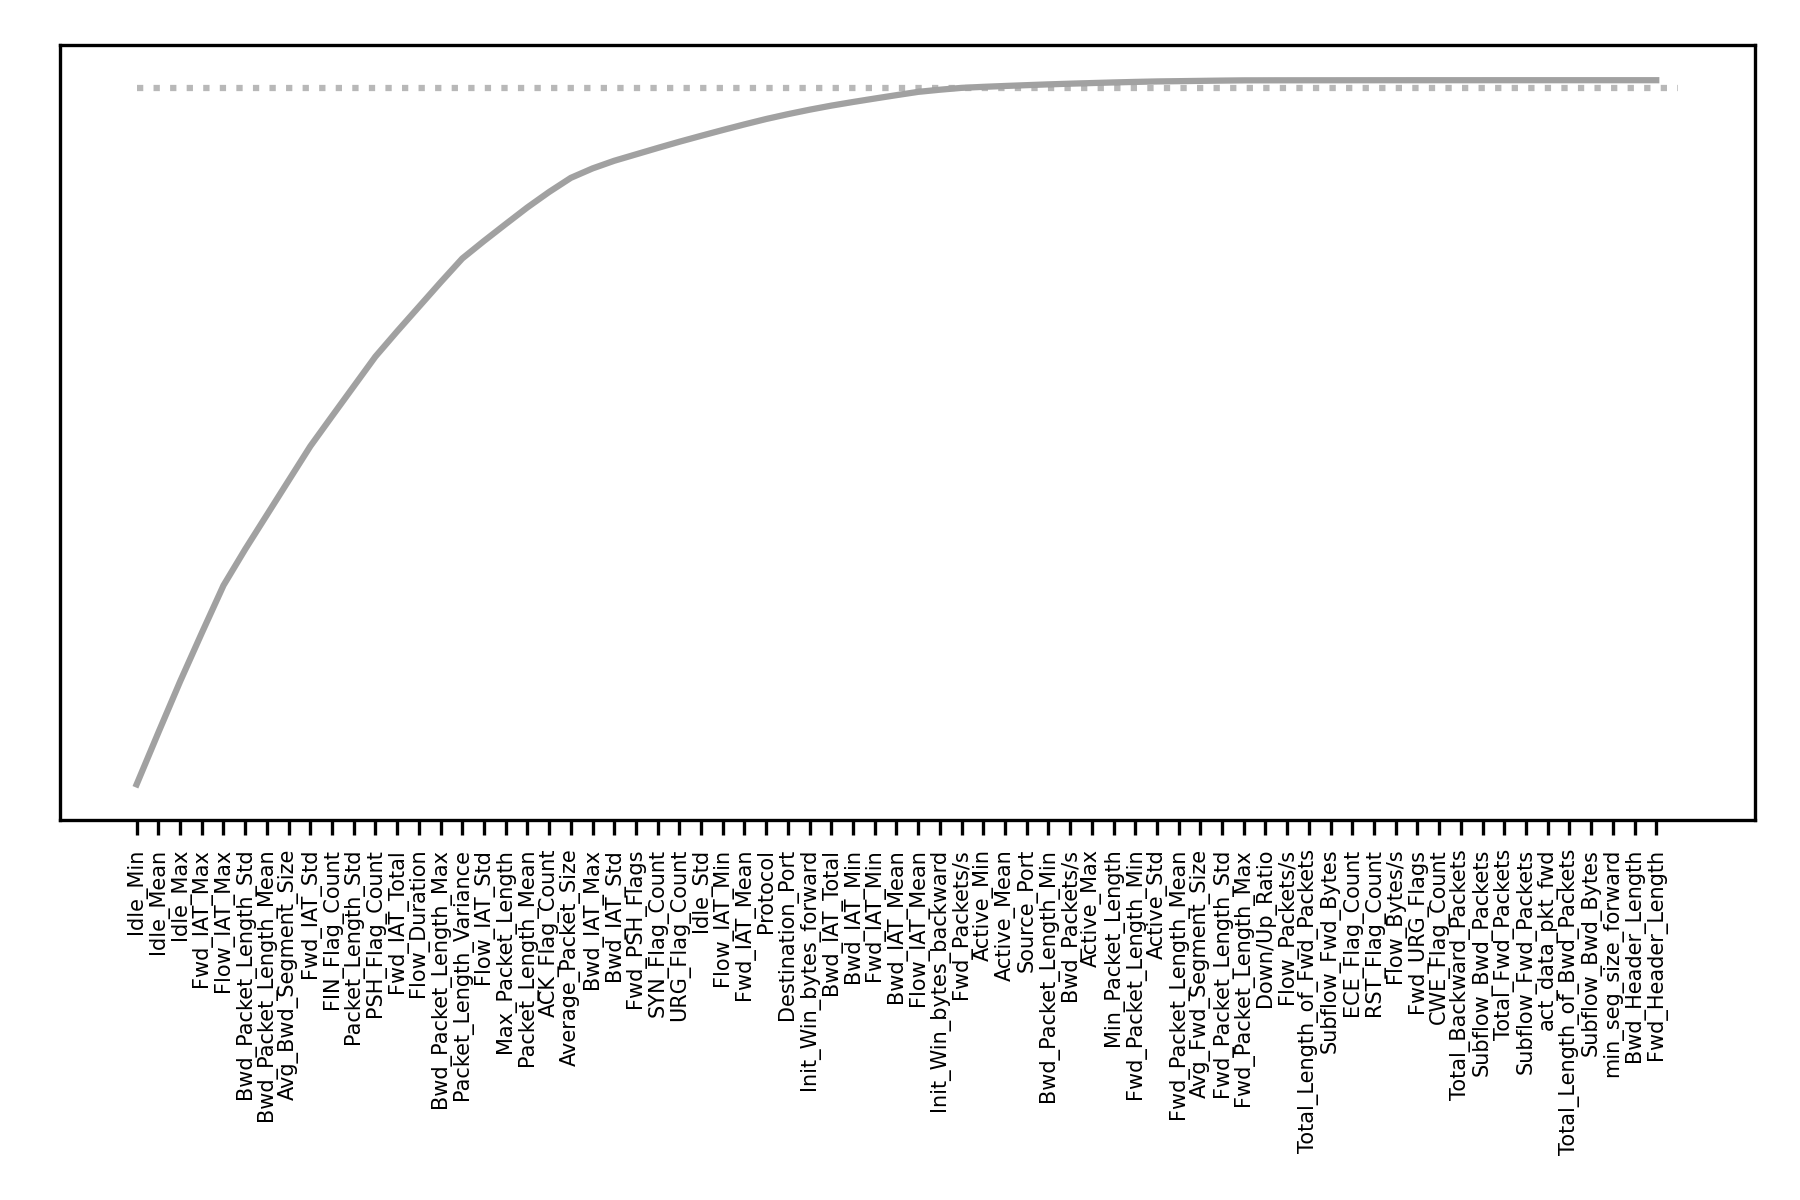
\includegraphics[scale=1]{assets/figures/chapter3/features99.png}
    \caption{CICIDS2017 Features Weight}
    \label{fig:features-weight}
\end{figure}

\noindent Table \ref{tab:features-weight} contains a list, along with the respective description of all the selected features, to summarize what was used in the training stage. For further data and statistics, see appendix \ref{app:net-features}.

\begin{table}[h!]
    \centering
    \begin{tabular}{l|l}
        \toprule 
        Feature & Description \\
        \midrule
        \rowcolor{black!10} \texttt{Destination\_Port} & Destination port number  \\
        \texttt{Protocol} & Protocol used \\
        \rowcolor{black!10} \texttt{Flow\_Duration} & Port Scan \\
        \texttt{Bwd\_Packet\_Length\_Max} & Maximum size of packet in backward direction \\
        \rowcolor{black!10} \texttt{Bwd\_Packet\_Length\_Mean} & Mean size of packet (backward direction) \\
        \texttt{Bwd\_Packet\_Length\_Std} & Standard deviation size of packet (backward direction) \\
        \rowcolor{black!10} \texttt{Flow\_IAT\_Mean} & Mean time between two packets sent in the flow \\
        \texttt{Flow\_IAT\_Std} & Standard deviation time between two packets sent in the flow \\
        \rowcolor{black!10} \texttt{Flow\_IAT\_Max} & Maximum time between two packets sent in the flow \\
        \texttt{Flow\_IAT\_Min} & Minimum time between two packets sent in the flow \\
        \rowcolor{black!10} \texttt{Fwd\_IAT\_Total} & Total time between two packets sent in the forward direction \\
        \texttt{Fwd\_IAT\_Mean} & Mean time between two packets sent in the forward direction \\
        \rowcolor{black!10} \texttt{Fwd\_IAT\_Std} & Standard deviation time between two packets (forward direction) \\
        \texttt{Flow\_IAT\_Max} & Maximum time between two packets sent in the flow \\
        \rowcolor{black!10} \texttt{Flow\_IAT\_Min} & Minimum time between two packets sent in the flow \\
        \texttt{Fwd\_IAT\_Total} & Total time between two packets sent in the forward direction \\
        \rowcolor{black!10} \texttt{Fwd\_IAT\_Mean} & Mean time between two packets (forward direction) \\
        \texttt{Fwd\_IAT\_Std} & Standard deviation time between two packets (forward direction) \\
        \rowcolor{black!10} \texttt{Fwd\_IAT\_Max} & Maximum time between two packets (forward direction) \\
        \texttt{Fwd\_IAT\_Min} & Minimum time between two packets sent in the forward direction \\
        \rowcolor{black!10} \texttt{Bwd\_IAT\_Total} & Total time between two packets (backward direction) \\
        \texttt{Bwd\_IAT\_Mean} & Mean time between two packets sent in the backward direction \\
        \rowcolor{black!10} \texttt{Bwd\_IAT\_Std} & Standard deviation time between two packets (backward direction) \\
        \texttt{Bwd\_IAT\_Max} & Maximum time between two packets sent in the backward direction \\
        \rowcolor{black!10} \texttt{Bwd\_IAT\_Min} & Minimum time between two packets (backward direction) \\
        \texttt{Fwd\_PSH\_Flags} & Number of times the PSH flag was set in packets (forward direction) \\
        \rowcolor{black!10} \texttt{Fwd\_Packets/s} & Number of forward packets per second \\
        \texttt{Max\_Packet\_Length} & Maximum length of a packet \\
        \rowcolor{black!10} \texttt{Packet\_Length\_Mean} & Mean length of a packet \\
        \texttt{Packet\_Length\_Std} & Standard deviation length of a packet \\
        \rowcolor{black!10} \texttt{Packet\_Length\_Variance} & Variance length of a packet \\
        \texttt{FIN\_Flag\_Count} & Number of packets with FIN \\
        \rowcolor{black!10} \texttt{SYN\_Flag\_Count} & Number of packets with SYN \\
        \texttt{PSH\_Flag\_Count} & Number of packets with PUSH \\
        \rowcolor{black!10} \texttt{ACK\_Flag\_Count} & Number of packets with ACK \\
        \texttt{URG\_Flag\_Count} & Number of packets with URG \\
        \rowcolor{black!10} \texttt{Average\_Packet\_Size} & Average size of packet \\
        \texttt{Avg\_Bwd\_Segment\_Size} & Average size observed in the backward direction \\
        \rowcolor{black!10} \texttt{Init\_Win\_bytes\_forward} & Total number of bytes sent in initial window (forward direction) \\
        \texttt{Init\_Win\_bytes\_backward} & Total number of bytes sent in initial window (backward direction) \\
        \rowcolor{black!10} \texttt{Active\_Min} & Minimum time a flow was active before becoming idle \\
        \texttt{Idle\_Mean} & Mean time a flow was idle before becoming active \\
        \rowcolor{black!10} \texttt{Idle\_Std} & Standard deviation time a flow was idle before becoming active \\
        \texttt{Idle\_Max} & Maximum time a flow was idle before becoming active \\
        \rowcolor{black!10} \texttt{Idle\_Min} & Minimum time a flow was idle before becoming active \\
        \bottomrule
    \end{tabular}
    \caption{CICIDS2017 (Selected) Features Weight and Description - most relevant to least relevant}
    \label{tab:features-weight}
\end{table}

\noindent The selected features are linked either to the packet length, to the flags or to the active/ idle time.

%\begin{figure}[h!]
%    \centering
%    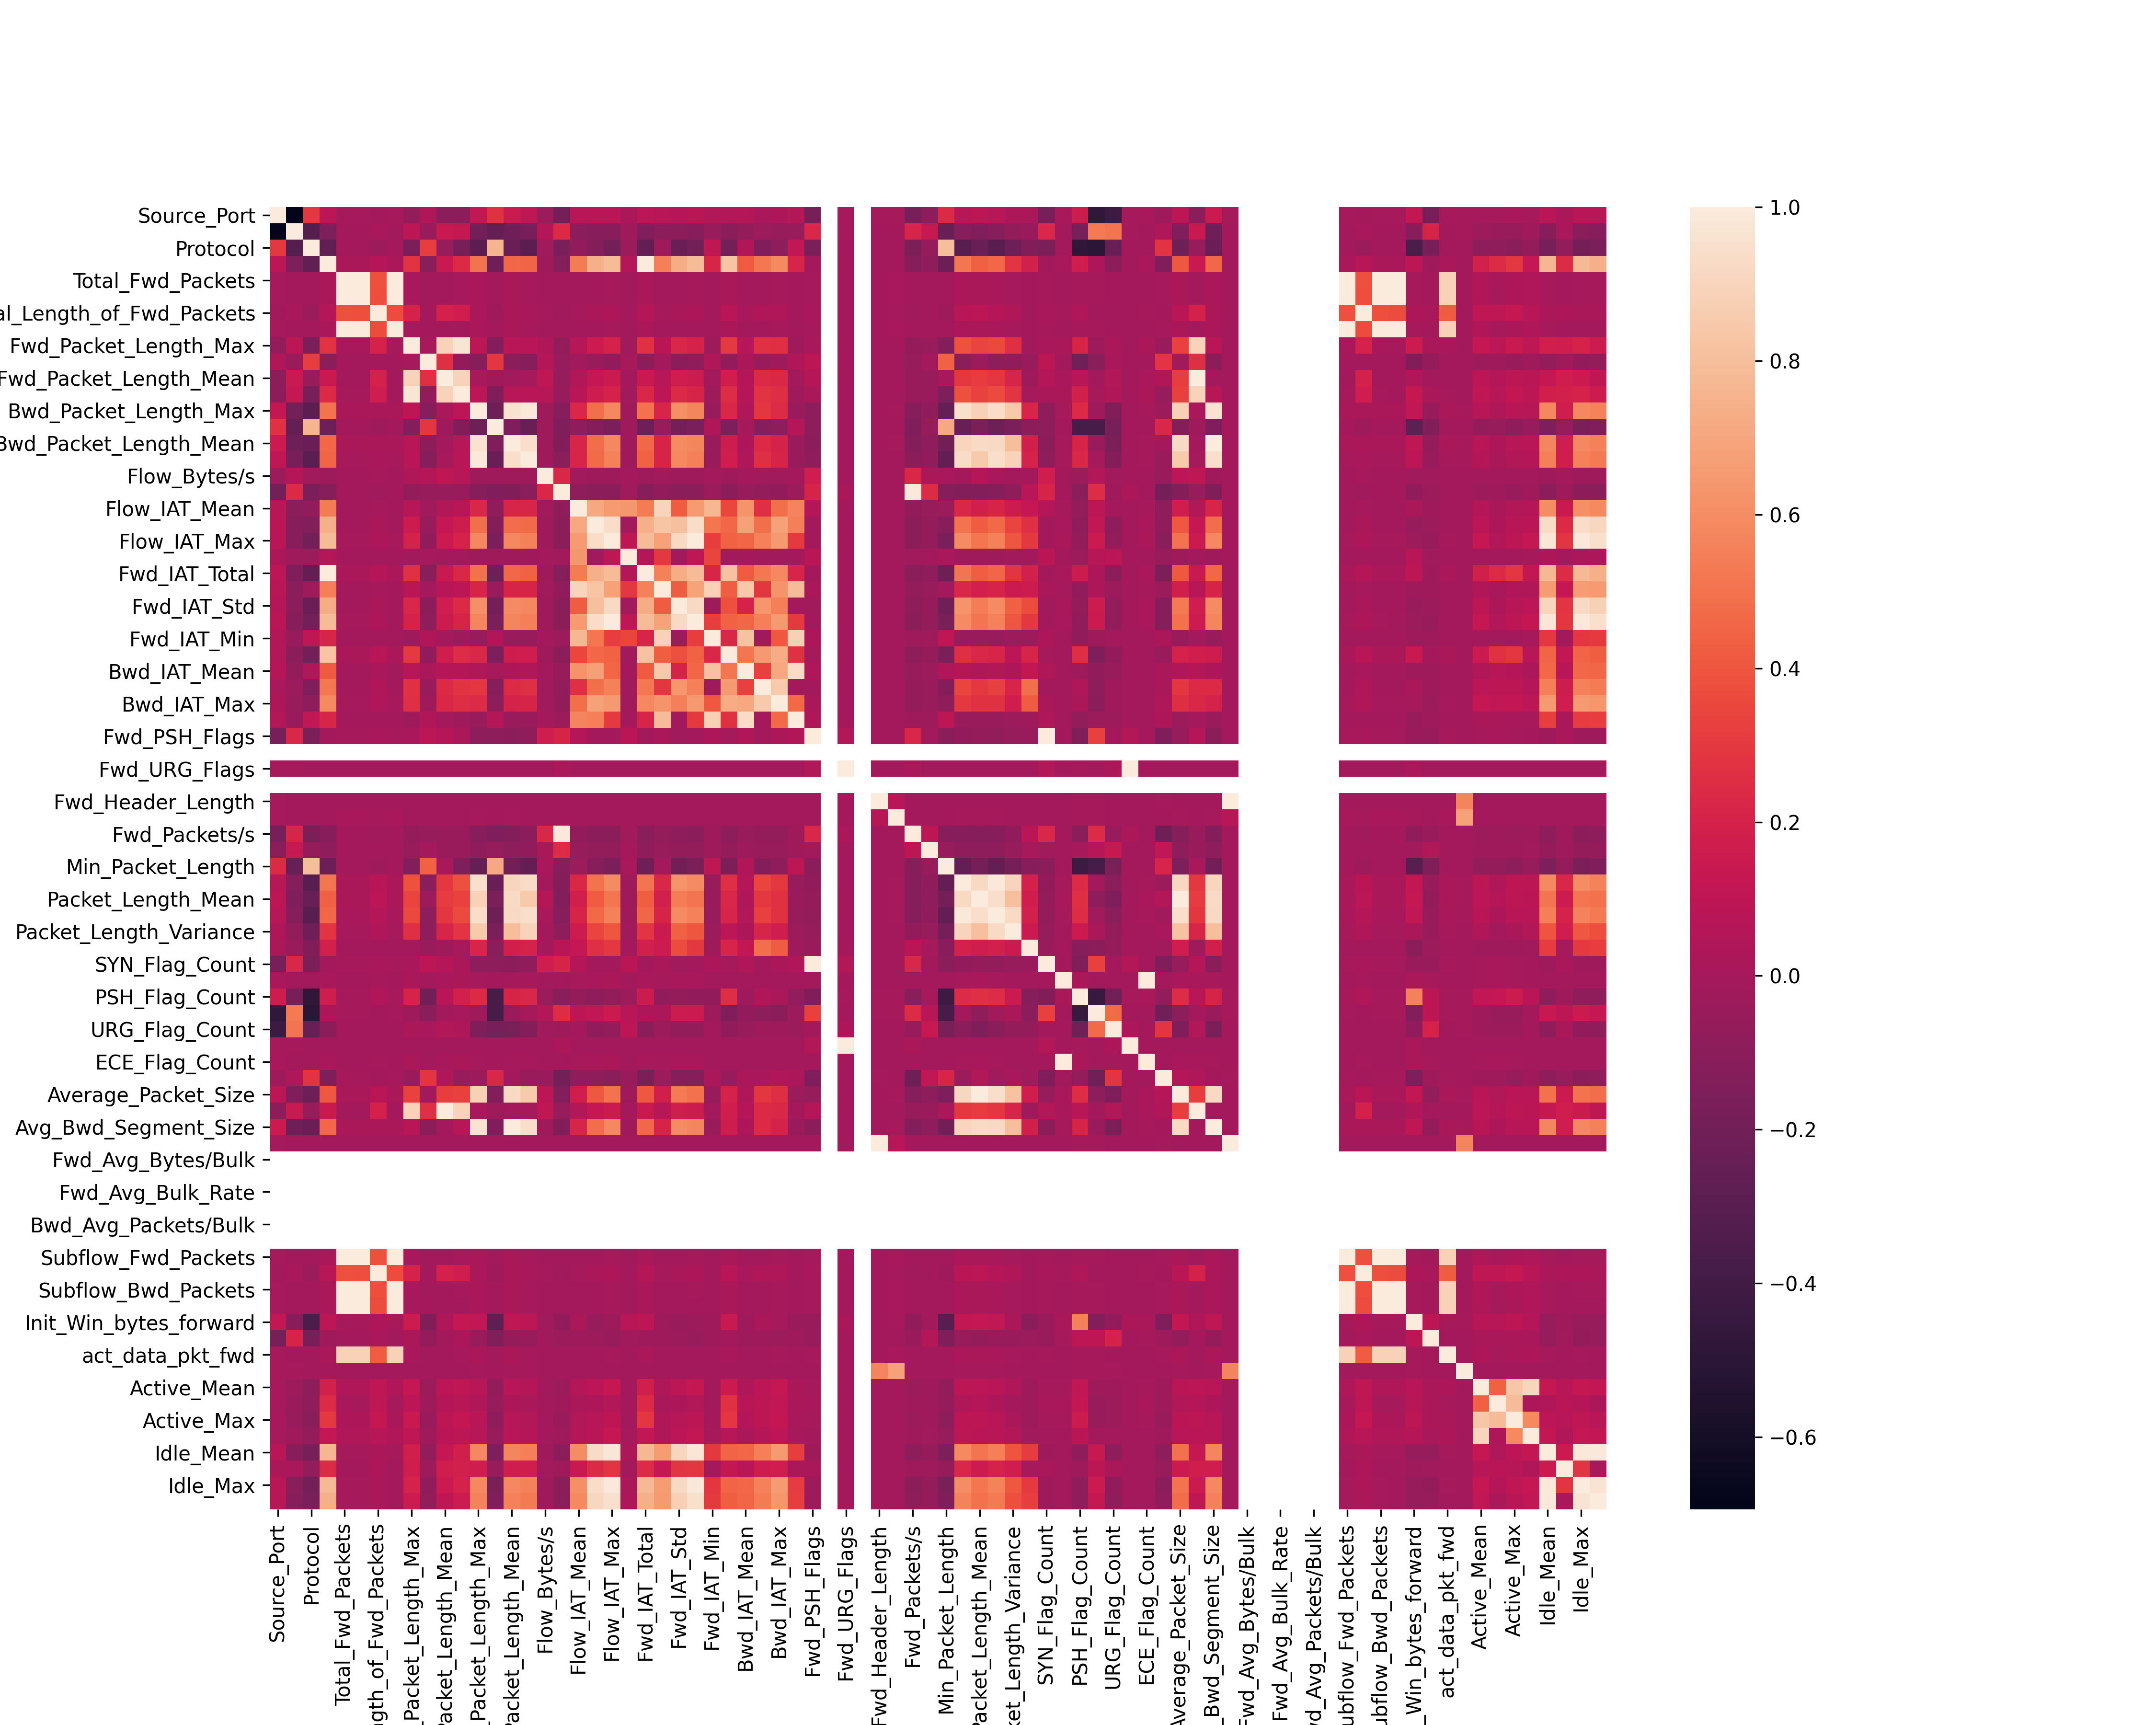
\includegraphics[scale=0.5]{assets/figures/chapter3/heatmap-all.png}
%    \caption{CICIDS2017 Feature Correlation Matrix (heatmap)}
%    \label{fig:feature-heatmap}
%\end{figure}

%----------------------------------------------------
% CLASSIFICATION
%----------------------------------------------------

\subsection{Classification}
\label{subsec:classification}

As disclosed in \ref{subsec:ml-algorithms}, the algorithm of choice for the classification stage is \textit{Random Forest}. This is a popular solution in classification problem and this is the reason why was adopted. It can be implemented with ease and can work with large datasets with no problem. The pre-processed dataset, after being split, was passed to the algorithm for training and testing. The resulting \textit{confusion matrix} can be observed in \ref{fig:confusion-matrix}.

\begin{figure}[h!]
   \centering
   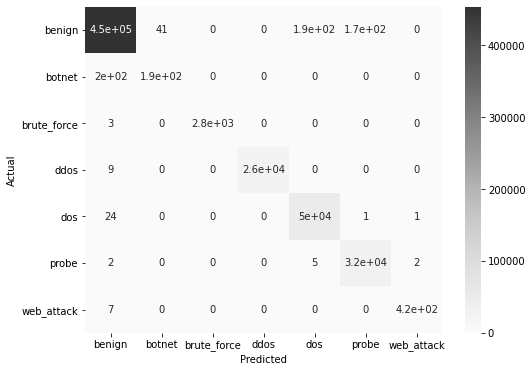
\includegraphics[scale=0.65]{assets/figures/chapter3/confusion_matrix.png}
   \caption{Confusion Matrix of the Random Forest model trained using CICIDS2017 dataset}
   \label{fig:confusion-matrix}
\end{figure}

\noindent This table layout allows visualization of the algorithm's performance. Each row of the matrix represents the instances in an \textit{actual} class, while each column represents the instances in a \textit{predicted} class. As the name suggests, the graph makes easier to see whether the model is confusing two classes: in this case the precision is remarkable, upholding the choice made.

%----------------------------------------------------
% NETWORK MONITOR
%----------------------------------------------------

\section{Network Monitor}
\label{sec:monitor-implementation}

The \textit{network monitor} is a key component of the system: it is used in both asynchronous and synchronous mode for analyzing the acquired packets, passing them to the model previously discussed. At this point the concept of \textit{flow} discussed in \ref{subsec:network-monitoring} comes in handy.

%----------------------------------------------------
% ML INTEGRATION
%----------------------------------------------------

\subsection{Flow Analysis}
\label{subsec:flow-analysis}

The \textit{Transport Layer} protocols relevant for the implementation are \gls{tcp} and \gls{udp}. As considered in \cite{Mozley2020}, \gls{udp} flows terminate on \textit{time out}, while \gls{udp} ones end with a \textit{time out}, but may also terminate via the FIN flag (last packet from sender), or RST flag (connection reset). The first packet in the flow is assumed to be in the forward direction, defining the source and, accordingly, the destination directions. \\ The code snippet below (from \texttt{app/Analyzer.py}) displays how packet reception is handled: if said packet doesn't belong to an existing flow, a new flow instance is created, otherwise it is necessary to check if it is a terminating packet. All current flows are stored in a dictionary, with the keys being the \textit{flow-ID}, and the value is the reference to the flow object. The features previously discussed are calculated after the flow is terminated and then passed to the classified in a \textit{feature vector}.

\begin{figure}[h!]
    \begin{code}[colback=white]{Flow Creation}
if packet.getFwdID() in current_flows.keys():
  flow = current_flows[packet.getFwdID()]
  if (packet.getTimestamp() - flow.getFlowStartTime()) > FlowTimeout:
    classify(flow.terminated())
    del current_flows[packet.getFwdID()]
    flow = Flow(packet)
    current_flows[packet.getFwdID()] = flow
  elif packet.getFINFlag() or packet.getRSTFlag():
    flow.new(packet, 'fwd')
    classify(flow.terminated())
    del current_flows[packet.getFwdID()]
    del flow
  else:
    flow.new(packet, 'fwd')
    current_flows[packet.getFwdID()] = flow
elif packet.getBwdID() in current_flows.keys():
  flow = current_flows[packet.getBwdID()]
  if (packet.getTimestamp() - flow.getFlowStartTime()) > FlowTimeout:
    classify(flow.terminated())
    del current_flows[packet.getBwdID()]
    del flow
    flow = Flow(packet)
    current_flows[packet.getFwdID()] = flow
  elif packet.getFINFlag() or packet.getRSTFlag():
    flow.new(packet, 'bwd')
    classify(flow.terminated())
    del current_flows[packet.getBwdID()]
    del flow
  else:
    flow.new(packet, 'bwd')
    current_flows[packet.getBwdID()] = flow
else:
  flow = Flow(packet)
  current_flows[packet.getFwdID()] = flow
\end{code}
\end{figure}

\lipsum[1-2]

\begin{figure}[h!]
    \begin{code}[colback=white]{Analyzer.py}
def classify(features):
print('Classifying...')
# Preprocess
f = features
features = [[np.nan if x in [np.inf, -np.inf]
                else float(x) for x in features]]

if np.nan in features:
    return

#features = normalisation.transform([features])
result = loaded_model.predict(features)

feature_string = [str(i) for i in f]
classification = [str(result[0])]

timestamp = [time.time() for k in classification]

readable = [time.ctime(time.time()) for j in classification]

if result != 'benign':
    print("MALICIOUS :: ", feature_string + classification + readable)
    # print(readable)

w.writerow(feature_string + classification)

mtt.writerow(timestamp + classification)

return feature_string + classification
\end{code}
\end{figure}

%----------------------------------------------------
% MONITORING PIPELINE
%----------------------------------------------------

\subsection{Monitoring Pipeline}
\label{subsec:monitoring-pipeline}

\textcolor{dimgray}{\lipsum[1-2]}

%----------------------------------------------------
% POC
%----------------------------------------------------

\section{Proof of Concept}
\label{sec:poc}

\textcolor{dimgray}{\lipsum}

%----------------------------------------------------
% TRAFFIC ACQUISITION
%----------------------------------------------------

\subsection{Traffic Acquisition}
\label{subsec:traffic-acquisition}

\textcolor{dimgray}{\lipsum}

%----------------------------------------------------
% TOPOLOGY
%----------------------------------------------------

\subsection{Topology}
\label{subsec:topology}

\textcolor{dimgray}{\lipsum[1]}

\begin{figure}[h!]
    \centering
    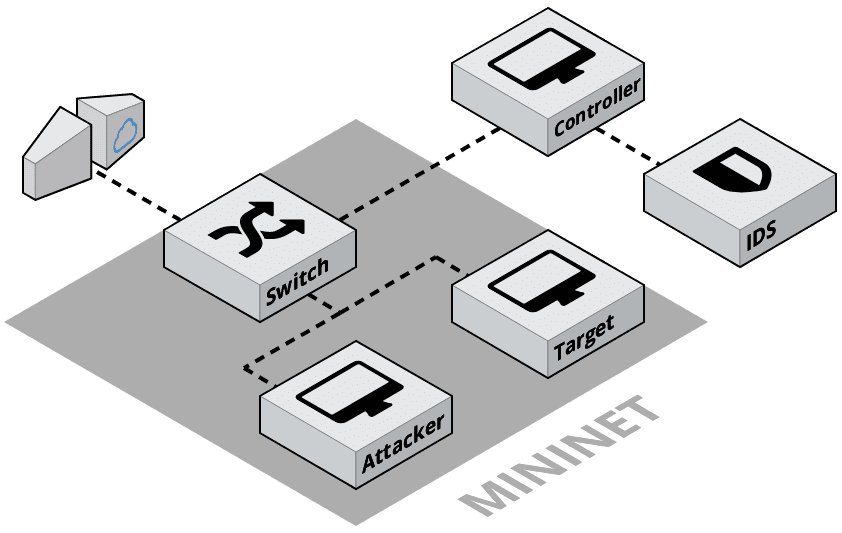
\includegraphics[scale=0.28]{assets/figures/chapter3/PoC_topology.png}
    \caption{Proof of Concept - Lab Topology}
    \label{fig:poc-topology}
\end{figure}

\textcolor{dimgray}{\lipsum[1]}
